\chapter{System Methodology and Implementation}
A privacy-preserving voting system requires deliberate choices at every layer of the stack, from smart contract logic to the off-chain processing pipeline. This chapter details the technology stack, smart contract design, off-chain batching workflow, and the rationale for local blockchain deployment. The design decisions at each stage are motivated by the dual requirements of voter anonymity and result integrity.
 
\section{Specifications for the Design}
 
The system is specified as a software-only prototype implementing the complete voting workflow within a local blockchain environment. Key functional requirements include: voter authentication through one-way identity hashing with no raw credential retained, off-chain vote buffering and shuffling prior to on-chain submission, smart contract enforcement of no-double-vote constraints, and a read-only results interface returning only aggregate tallies. Non-functionally, the system must deploy on a local \gls{evm}-compatible chain without external dependencies and remain modular enough to migrate to a public chain through configuration changes alone.

\begin{figure}[htbp]
    \centering
    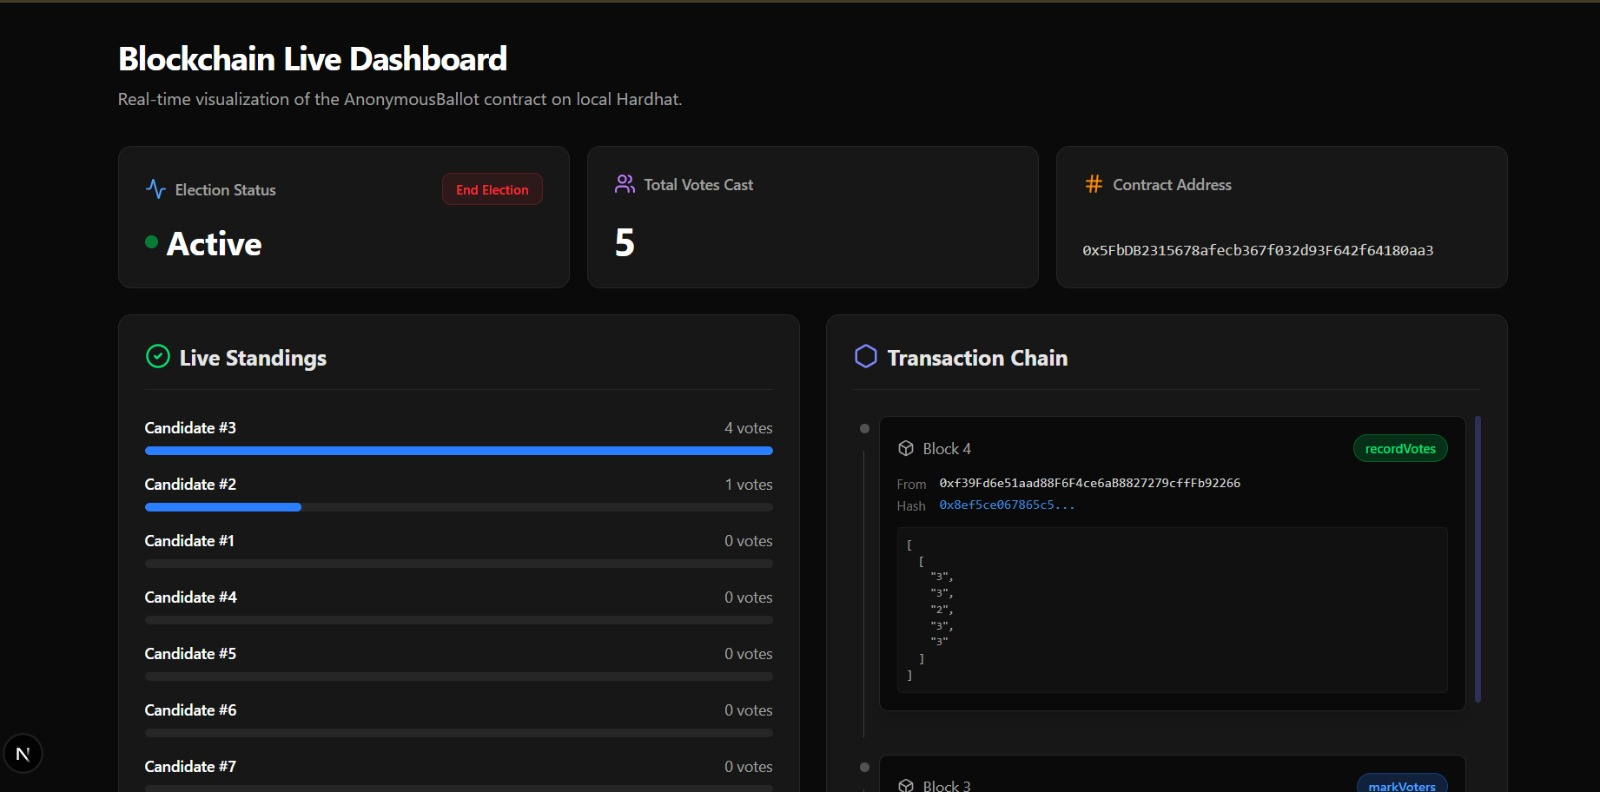
\includegraphics[width=0.8\linewidth]{Chapter3/3(1).jpeg}
    \caption{Blockchain live dashboard}
    \label{fig:Design implementation}
\end{figure}

 
\section{Technology Stack and Pre-Analysis}
 
\subsection{Threat Model}
 
Two primary threat classes were identified prior to design. A \textit{linkage attack} attempts to correlate on-chain data to reconstruct voter-to-candidate mappings; this is mitigated by separating identity and candidate submissions into two independently shuffled arrays \cite{Alsadi2024}. A \textit{double-vote attack} attempts to reuse an identity hash; this is defeated by the smart contract's spent-key register, which rejects any batch containing a previously used hash.
 
\subsection{Technology Stack}
 
A JavaScript single-page application provides the voter-facing \gls{ui} in two modes: a standard visual ballot and a voice-guided agentic flow using the Web Speech \gls{api}. A lightweight \gls{rest} backend manages the vote buffer, shuffle module, and relayer. The smart contract is written in Solidity and deployed to a local \gls{evm}-compatible development chain, with the relayer as the sole actor submitting batched transactions via \gls{rpc}.
 
\section{Design Methodology}
 
\subsection{Smart Contract Logic}
 
The contract follows a three-phase state machine: \texttt{Registration}, \texttt{Voting}, and \texttt{Closed}. It exposes two write functions called sequentially by the relayer: \texttt{markIdentitiesUsed(bytes32[] identities)}, which checks each hash against the spent-key register and reverts on any duplicate, and \texttt{recordVotes(uint8[] candidateIds)}, which increments tally counters. A public \texttt{getResults()} function returns aggregate counts without any per-voter data.
 
\subsection{Off-Chain Processing and Design Equations}
 
Votes are buffered as (hashed identity, candidate \gls{id}) pairs. When the buffer reaches threshold $\theta$, the candidate \gls{id} array is shuffled using a Fisher-Yates permutation before submission. The identity hash is computed as:
\begin{equation}
    h_i = H(v_i), \quad H : \{0,1\}^* \rightarrow \{0,1\}^{256}
    \label{eq:identity_hash}
\end{equation}
where $H$ is \gls{sha}-256. The flush condition is $n \geq \theta$, and the shuffle draws a permutation $\pi$ uniformly from $\mathcal{S}_\theta$, ensuring no positional correspondence between the identity and candidate arrays on-chain \cite{Wang2023}.
 
\begin{figure}[htb]
\centering
    % \includegraphics[scale=0.8]{Figures/offchain_workflow}
    \caption{Off-chain batching and shuffle workflow prior to on-chain submission}
    \label{fig:offchain_workflow}
\end{figure}
 
Figure~\ref{fig:offchain_workflow} illustrates the five-step off-chain workflow: vote submission to the buffer, threshold check, Fisher-Yates shuffle of the candidate column, relayer submission of the identity array, and relayer submission of the shuffled candidate array. The buffer is cleared after each successful batch, and the on-chain record carries no structural information that could reconstruct vote-to-voter mappings.
 
\section{Local Chain Rationale}
 
Deployment on a local chain rather than a public network eliminates dependencies on external validators, removes gas fee uncertainty, and restricts on-chain data visibility to participants within the deployment boundary. These properties make the system viable for edge environments with limited connectivity. The modular architecture ensures that migrating to a public or permissioned chain in a future phase requires only reconfiguration of the relayer's \gls{rpc} target and the contract deployment address.
 
This chapter has presented the methodology underlying the proposed system, covering the technology stack, contract design, off-chain shuffle workflow, and local chain deployment rationale. The Fisher-Yates shuffle combined with two-stage batch submission implements the unlinkability property central to the privacy design. The following chapter presents the implementation details and test results, evaluating tally correctness, double-vote prevention, and the effectiveness of the shuffle in breaking observable ordering patterns.
 